%-*- coding: UTF-8 -*-
% report.text
% 机器学习结课项目报告 
\documentclass[UTF8]{ctexart}
\usepackage{graphicx}
\usepackage{graphics}
\usepackage{float}
\usepackage[colorlinks,linkcolor=blue]{hyperref}
\usepackage{listings}
\usepackage{xcolor}
\usepackage{geometry}
\usepackage{setspace}
\usepackage{fancyhdr}
\usepackage{subfigure}
\usepackage{booktabs}
\title{机器学习实验报告}
\author{葛松}
\date{\today}

\geometry{a4paper,left=2cm,right=2cm,top=3cm,bottom=2cm}

\pagestyle{fancy}
\fancyhf{}
\rhead{\thepage}
\lhead{\leftmark}

% 代码样式
\lstset{
    frame=L,
    language=Python,
    aboveskip=1mm,
    belowskip=1mm,
    showstringspaces=false,
    columns=flexible,
    basicstyle={\small\ttfamily},
    numbers=left,
    keywordstyle=\color[RGB]{40,40,255}, 
    commentstyle=\itshape\color{orange},
    stringstyle=\color[RGB]{0.58,0,0.82},
    backgroundcolor=\color[RGB]{245,245,244},  
    breaklines=true,
    breakatwhitespace=true,
    tabsize=4,
%   xleftmargin=\parindent,
%   numbersep=5pt,
}

\begin{document}
\thispagestyle{empty}
\begin{figure}[htb]
    \centering
    
\includegraphics[width=3in]{asset/华中科技大学.png}
\end{figure}

\begin{center}
    \fangsong
    \zihao{0}项目开发报告
\end{center}



\vspace*{20mm}
\begin{center}
    \zihao{4}\textbf{题目}:\underline{\makebox[15em]{疫情期间网民情绪识别}}
\end{center}

\vspace*{70mm}

\begin{center}
    \zihao{5}\textbf{课程名称}: \underline{\makebox[15em]{机器学习}}
    
    \zihao{5}\textbf{专业班级}: \underline{\makebox[15em]{CS1703}}

    \zihao{5}\textbf{学\qquad 号}: \underline{\makebox[15em]{U201714668}}
    
    \zihao{5}\textbf{姓\qquad 名}: \underline{\makebox[15em]{葛松}}
    
    \zihao{5}\textbf{指导教师}: \underline{\makebox[15em]{李玉华}}
    
    \zihao{5}\textbf{报告日期}: \underline{\makebox[15em]{\today}}
\end{center}

\vspace*{50mm}

\begin{center}
    \zihao{4}计算机科学与技术学院
\end{center}
\newpage
\thispagestyle{empty}
\tableofcontents
\newpage
\setcounter{page}{1}
\section{疫情期间网民情绪识别}
\subsection{项目目的}
\begin{enumerate}
    \item 掌握文本处理的基本方法
    \item 理解不同算法结果的差异性
    \item 掌握对程序运行结果的评价方法
\end{enumerate}

% \vspace*{5mm}

\subsection{项目内容}
\begin{enumerate}
    \item 根据  \lstinline{train.csv} 文件中的微博数据,设计算法对  \lstinline{test.csv} 文件中的 4500 条微
    博内容进行情绪识别,判断微博内容是积极的(1)、消极的(-1)还是中性的
    (0)。
    \item 通过混淆矩阵对算法的结果进行评价
    \item 使用多种模型对问题进行处理,并进行对比
\end{enumerate}

% \vspace*{5mm}
% \newpage
\subsection{问题分析}
所有的文本分析问题,基本都包括以下几个部分,下文将对这几个方面对问题进行分析
\begin{quote}
    \begin{itemize}
        \item 数据预处理,根据数据的特性进行清洗
        \item 数据转换,即将文本转化为可计算的的值
        \item 模型训练,将转换后的数据输入模型中进行训练,并对测试目标进行预测
    \end{itemize}
\end{quote}

\subsubsection{数据预处理}
由于本次项目的数据为微博真实数据,并且没有进行任何预处理,所以需要先对数据进行清洗以便后续工作。
基本的预处理包括以下几个步骤
\begin{quote}
    \begin{itemize}
        \item 中文分词
        
        由于中文与英文不同,不像英文一样自然以空格分割,而是全部连接在一起的。
        所以需要对中文进行单词的分割。也即\textit{中文分词}。以便以单词为单位进行后续的分析。
        中文分词在业内已经有比较成熟的解决方案,相关的工具包也比较丰富,
        如\lstinline{jieba}分词,清华大学的\lstinline{THULAC},以及MIT的\lstinline{SnowNLP}
        \item 去除停用词
        
        所谓\textit{停用词}即为一些无法表征特别多信息的词语,如\textit{你},\textit{我}, \textit{他},
        以及一些标点符号等等。这些词语出现的次数可能非常多,但是却无法带给我们有效的信息,反而会影响我们
        后续的计算,所以需要进行去除。在github上可以找到很多已经归纳好的停用词列表,可以通过综合多个停用词列
        表来得到一个更大的集合,从而增加去除的准确度。同时我们需要针对微博数据的特点进行针对性的处理,在给出的数据中
        很多情况下,一句话都包含有诸如\textit{@账号名},又或是\textit{话题名}等信息,如
        \textit{//@新疆发布:\#众志成城打赢疫情防控阻击战\#众志成城防疫情,我在新疆,我承诺!}
        中的\textit{@新疆发布}就是账号名,并不是评论本身。
        \item 去除频数较小的词(可选)
        
        去除停用词之后可能还会有一些频数非常小的词语,其本身出现的次数不多,但是这类词语会极大地增加我们的词语集合,如果采用\lstinline{one-hot}
        编码,将会使我们的向量变得非常庞大,难以计算(本次实验中去除后的词语集合达到了2万多个)。幸运的是,在训练词向量的过程中,相关的函数基本上都会提供
        一个可选的参数来设置词语的最小出现次数,非常方便的解决了这个问题。
    \end{itemize}
\end{quote}

\subsubsection{数据转换}
所有的机器学习问题都要面临的一个问题就是如何将采集到的数据变为可以计算的数字,而针对文本处理,基本有以下几种常用的转换方法
\begin{quote}
    \begin{itemize}
        \item 独热编码(\lstinline{one-hot})
            
            即将每一个句子转化为一个长度为词库大小的向量,当包含这个词语时就将对应位置设置为1,否则为0,但是由于词库往往非常大,会导致
            生成的数据非常庞大,并且非常稀疏,导致计算效果不佳
        \item 整数编码
            
        将每一个词语用唯一的数字标示进行标示,整个句子将表示为词语标识的序列,常常需要对句子的长度进行统一,常见于简单实现的神经网络模型中
        
        \item 词袋模型(\lstinline{bag-of-word})
        
        与独热编码唯一的不同就是保存了出现次数,而不仅仅为0,1值

        \item 词嵌入(\lstinline{word-embedding})
        
        通过\lstinline{CBOW}或者\lstinline{Skip-Gram}等模型,将每一个词语转化为指定维度的向量表示,生成出的向量则包含了该词语的语义信息。
        相近的词语在高维空间中所对应的距离往往也比较小。
        再通过句子所包含的所有词的词向量来获取该句子所对应的向量(通常为直接将每一个词语的向量相加)。相较于前面的几种方法,词嵌入有压缩语义信息、
        向量长度较短等优点。
    \end{itemize}
\end{quote}

而在本次项目中,为了提高准确率,分别针对普通线性模型,如\lstinline{svm}、\lstinline{logistics}回归,以及简单的神经网络,分别采用了词嵌入以及整数编码的方法
,同时辅以\lstinline{PCA}等降维方法,使得训练时间进一步减小。

\subsubsection{模型训练以及评价}
在实际运行过程中,实际上尝试了非常多种方法,如\lstinline{KNN}、\lstinline{SVM}、\lstinline{Logistic}回归。亦或是直接调用他人写好的文本分析库
如\lstinline{SnowNLP},以及一些神经网络等等。但是由于正确率等原因,最终还是选择了\lstinline{logistic}回归,\lstinline{SVM}以及简单的神经网络
作为本报告介绍的对象。

对于最终效果的评价,采用了题目中所要求的三种评价指标,分别为
\begin{quote}
    \begin{itemize}
        \item \lstinline{Precision} (精准率)
        \item \lstinline{Recall} (召回率)
        \item \lstinline{F1-score} (F1)分数
    \end{itemize}
\end{quote}

分别对不同模型的预测结果给出相应的评价
\newpage
\subsection{设计与分析}
该部分与问题分析部分一一对应,分别介绍不同阶段的设计与主体代码,整体程序流程图如下图所示

\begin{figure}[htb]
    \centering
    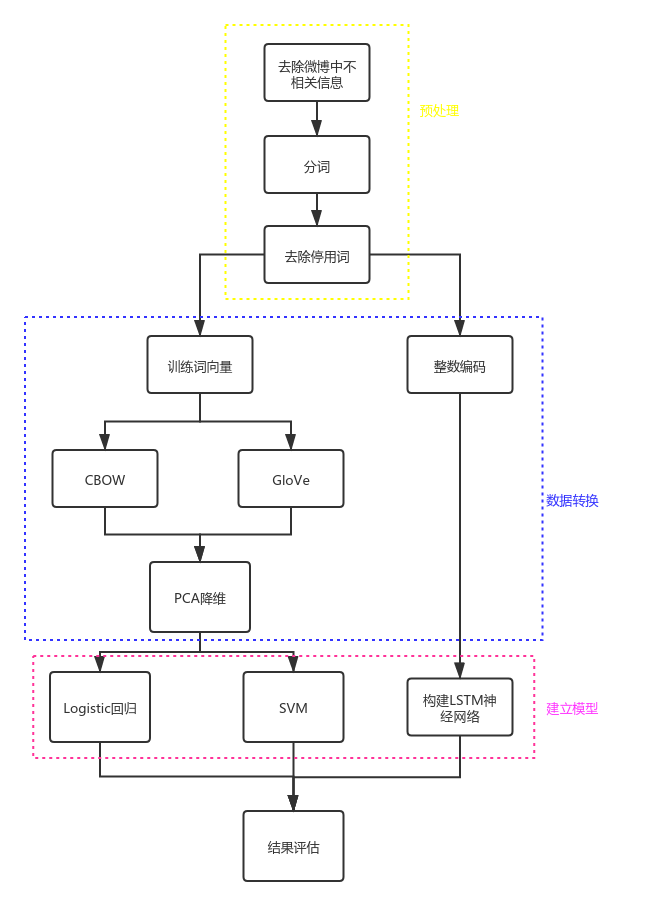
\includegraphics[width=4in]{asset/流程图.png}
    \caption{数据清洗结果} %最终文档中希望显示的图片标题
    % \label{Fig.main2} %用于文内引用的标签
\end{figure}

\newpage
\subsubsection{数据预处理}
\subsubsection*{分词}
在本次实验中,我们采用业界比较成熟的分词工具\lstinline{jieba}来对数据进行分词,通过以下函数可以非常方便的将中文句子分割为一个个的单词
\begin{quote}
    \begin{lstlisting}
    words = jieba.lcut(sentence, HMM=False)
    \end{lstlisting}
\end{quote}

\subsubsection*{去除停用词}
我们采用github上一个非常齐全的停用词列表\href{https://github.com/goto456/stopwords}{仓库}来构成本项目所用到的停用词表。
包括哈工大停用词表,百度停用词表等等。
同时定义以下函数来综合多个停用词表。
\begin{quote}
    \begin{lstlisting}[]
    def makeStopWord():
        stopword = set()
        for file in listdir('stopwords'):
            if file.endswith("txt"):
                with open(f'stopwords/{file}') as f:
                    lines = f.readlines()
                    for line in lines:
                        words = jieba.lcut(line, cut_all=False)
                        for word in words:
                            stopword.add(word.strip())
        return stopword
    \end{lstlisting}
\end{quote}

\subsubsection*{去除账号名等不相关数据}
观察微博数据中账号名以及话题出现的模式,发现可以通过正则匹配来进行去除,如下代码便使用了正则表达式来匹配多种可能的情况,去除不相关数据
\begin{quote}
    \begin{lstlisting}
    def clean_redundant(comment):
        comment = re.sub('#.*?#', '', comment)
        comment = re.sub('//@.*?:', '', comment)
        comment = re.sub('//@.*?:', '', comment)
        comment = re.sub('//.*?:', '', comment)
        comment = re.sub('//.*?:', '', comment)
        comment = re.sub('【.*?】', '', comment)
        comment = re.sub('《.*?》', '', comment)
        comment = re.sub('//.*?//', '', comment)
        comment = re.sub('@.*?:', '', comment)
        comment = re.sub('@.*?:', '', comment)
        comment = re.sub('『.*?』', '', comment)
        comment = re.sub(r'\d', '', comment)
        return comment
    \end{lstlisting}
\end{quote}

在经过分词、去除停用词、以及针对微博特性的清洗之后,原数据变为了易于处理的单词格式,如下图所示


\begin{figure}[htb]
    \centering
    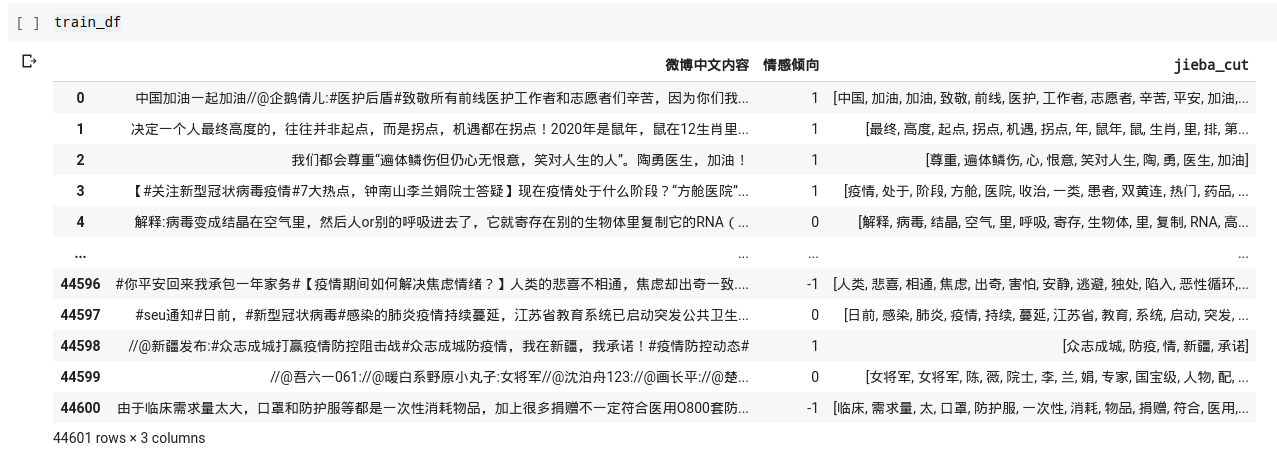
\includegraphics[width=6in]{asset/数据清洗.png}
    \caption{数据清洗结果} %最终文档中希望显示的图片标题
    % \label{Fig.main2} %用于文内引用的标签
\end{figure}

需要注意的是,经过了上述处理之后,一些句子可能会变为空,针对这些句子也进行了去除处理,但好在这种情况非常少,不会有很大的影响。

\subsubsection{数据转换}
以下分别介绍项目中所用的词嵌入以及整数编码的方法
\subsubsection*{词嵌入}
词嵌入有多种不同的模型,其中\lstinline{GloVe}模型以及\lstinline{CBOW}模型是效果比较好的两种模型。通过将分词好的数据输入到对应模型中进行训练
可以得到针对该数据集合的词向量。本项目中两种模型均进行了尝试。
\begin{itemize}
    \item \lstinline{CBOW}模型
    
    \lstinline{CBOW}模型可以通过\lstinline{word2vec}包来非常方便的进行训练,如下述代码所示
    \begin{lstlisting}[]
    from itertools import chain
    from gensim.models import Word2Vec
    from gensim.models.word2vec import LineSentence
    corpus = [" ".join(x) for x in chain(train_df.jieba_cut, test_df.jieba_cut)]
    # 将语料库写入文件
    with open('corpus.txt' , 'w') as f:
    for i in corpus:
        f.write(i + "\n")
    # 开始训练
    # 维度为800
    model = Word2Vec(LineSentence('./corpus.txt'), size=1000, window=5, min_count=5, workers=8)
    \end{lstlisting}
    得到\lstinline{model}后便可以通过\lstinline{model[word]}的方式来获取某一个词语所对应的词向量。而具体训练的效果可以通过查看某一个词语的
    最相近词来间接查看。我们以\textit{关心}为例,查看其最近的几个词语,如下图所示
    \begin{figure}[htb]
        \centering
        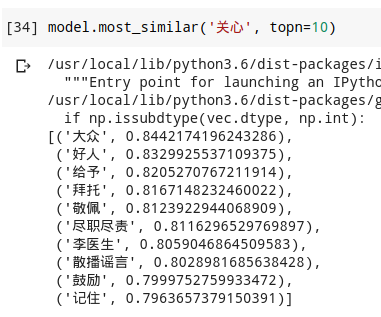
\includegraphics[width=3in]{asset/关心word2vec.png}
        \caption{与\textit{关心}最近的词语} %最终文档中希望显示的图片标题
        % \label{Fig.main2} %用于文内引用的标签
    \end{figure}
    可见训练结果还是比较理想的
    \newpage
    \item \lstinline{GloVe}模型
    
    与\lstinline{CBOW}模型有标准Python实现不同,斯坦福的\lstinline{GloVe}模型的官方实现为C语言,
    所以需要从github克隆其\href{https://github.com/stanfordnlp/GloVe}{仓库},并修改shell脚本中的配置内容,再进行训练。
    脚本内容以及训练过程如下图所示
    \begin{figure}[htb]
        \centering
        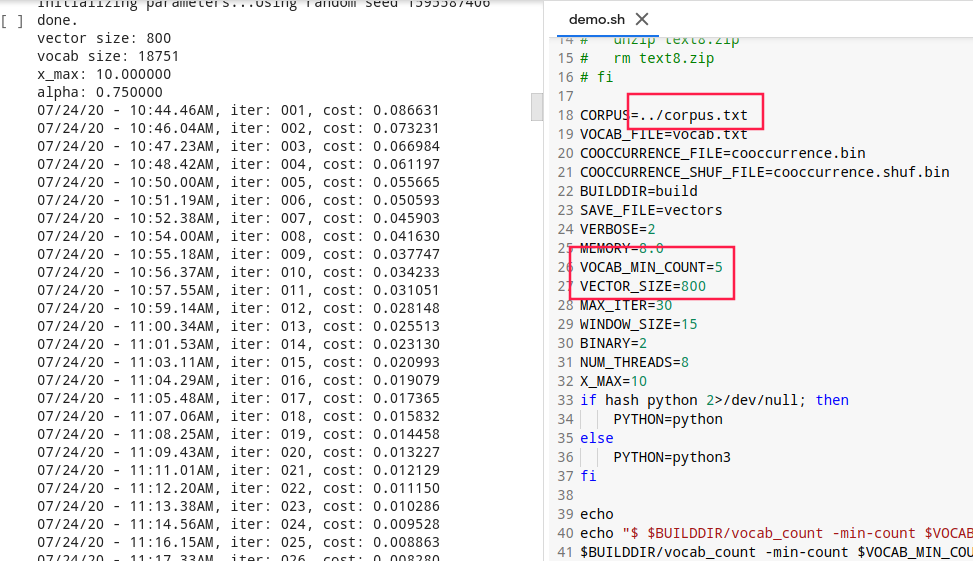
\includegraphics[width=6in]{asset/GloVe训练过程.png}
        \caption{GloVe训练过程} %最终文档中希望显示的图片标题
        % \label{Fig.main2} %用于文内引用的标签
    \end{figure}

    其中维数也设置为800。
    同样以\textit{关心}为例,查看其最近的几个词语,如下图所示
    \begin{figure}[htb]
        \centering
        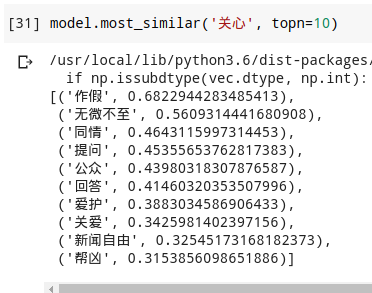
\includegraphics[width=3in]{asset/关心glove.png}
        \caption{与\textit{关心}最相近的词语} %最终文档中希望显示的图片标题
        % \label{Fig.main2} %用于文内引用的标签
    \end{figure}
    可见效果也还不错

    \newpage
    上述两个模型均可以在一定程度上实现词语的嵌入。但是得到的结果向量维度还是非常高。这里我们采用了PCA降维的方法来将其映射到低维空间,且尽量不损失信息。
    从而方面后续计算
    
    首先需要计算不同维度下的信息损失程度,由此再确定要将其降维到多少,具体代码如下所示
    \begin{lstlisting}[]
    import matplotlib.pyplot as plt
    from sklearn.decomposition import PCA
    from sklearn import metrics
    
    # 载入数据
    df = data
    y = df.iloc[:,0]
    x = df.iloc[:,1:]
    ##原始维度为800
    n_components = 800
    pca = PCA(n_components=n_components)
    pca.fit(x)
    #打印 pca.explained_variance_ratio_

    ##PCA作图
    plt.figure(1, figsize=(12, 8))
    plt.clf()
    plt.axes([.2, .2, .7, .7])
    plt.plot(pca.explained_variance_, linewidth=2)
    plt.axis('tight')
    plt.xlabel('n_components')
    plt.ylabel('explained_variance_')
    plt.show()
    \end{lstlisting}
    结果如下图所示
    \begin{figure}[htb]
        \centering
        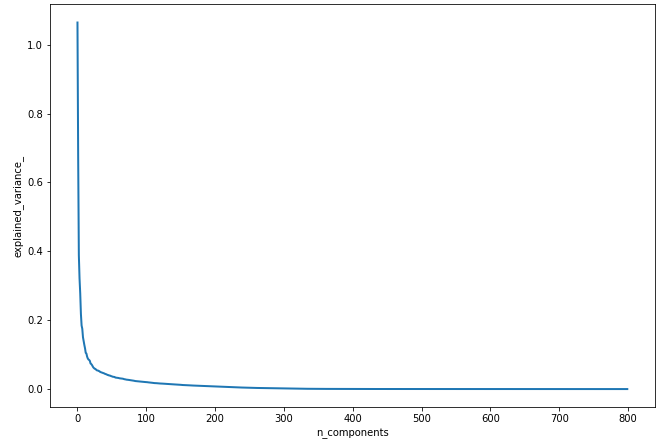
\includegraphics[width=4in]{asset/pca降维分析.png}
        \caption{PCA降维} %最终文档中希望显示的图片标题
        % \label{Fig.main2} %用于文内引用的标签
    \end{figure}
    可见在200维的时候,既达到了大幅降低了维度的目的,同时也基本没有损失信息。
\end{itemize}
\newpage
\subsubsection*{整数编码}
整数编码的方法在本项目中主要用于实现简单的LSTM神经网络,使用了\lstinline{tensorflow}作为具体实现,而\lstinline{tensorflow}也提供了相关的函数进行
整数编码。

其中需要确定每一个句子的长度,不足的补0,多余的部分裁去。通过对清洗后的句子的长度绘制出分布图,如下图所示
\begin{figure}[htb]
    \centering
    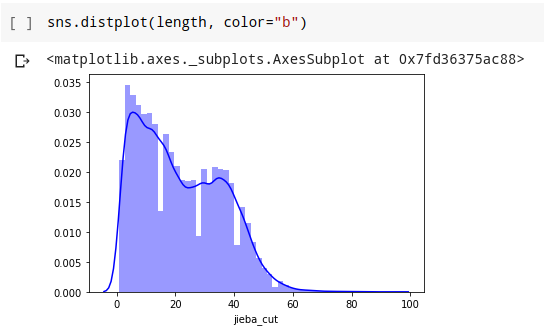
\includegraphics[width=5in]{asset/句子长度.png}
    \caption{句子长度分布} %最终文档中希望显示的图片标题
    % \label{Fig.main2} %用于文内引用的标签
\end{figure}

可以发现长度设置成60比较合适
\newpage
\subsubsection{模型训练}
本报告选出了实际运行结果相对较好的几种模型进行介绍,分别有

\begin{quote}
    \begin{itemize}
        \item \lstinline{Logistic}
        \item \lstinline{SVM}
        \item \lstinline{LSTM}网络
    \end{itemize}
\end{quote}

其中\lstinline{Logistic}以及\lstinline{SVM}这两种模型可以通过调用\lstinline{sklearn}包中的默认实现,输入上文所提到的\lstinline{PCA}降维后的
数据进行训练即可。通过多次训练,调整参数找到较优解。具体代码如下所示
\begin{quote}
    \begin{lstlisting}[]
    # 逻辑斯特回归
    from sklearn.linear_model import LogisticRegression
    lr = LogisticRegression(C=0.001, random_state=1, max_iter=10000)
    lr.fit(X_train, y_train)
    # 分别计算训练集以及测试集的正确率
    lr.score(X_train, y_train)
    lr.score(X_test, y_test)

    # 支持向量机
    from sklearn import svm
    clf = svm.SVC(C=0.1, probability=True, cache_size=8192)
    clf.fit(X_train, y_train)
    # 分别计算训练集以及测试集的正确率
    clf.score(X_train, y_train)
    clf.score(X_test, y_test)
    \end{lstlisting}
\end{quote}

而\lstinline{LSTM}模型通过\lstinline{tensorflow}可以非常方便的实现,代码如下所示
\begin{quote}
    \begin{lstlisting}[]
    ## 两层LSTM,中间用Dropout层避免过拟合
    model = tf.keras.Sequential([
        tf.keras.layers.Embedding(vocab_size, embedding_dim),
        tf.keras.layers.LSTM(embedding_dim),
        tf.keras.layers.Dropout(0.4),
        tf.keras.layers.Dense(embedding_dim, activation='relu'),
        tf.keras.layers.Dropout(0.4),
        tf.keras.layers.Dense(3, activation='softmax')
    ])
    model.compile(loss='sparse_categorical_crossentropy', optimizer='adam', metrics=['accuracy'])
    ## 遍历数据10次
    num_epochs = 10
    history = model.fit(X_train_padded,
                        train_df["情感倾向"]+1,
                        epochs=num_epochs,
                        validation_data=(X_validation_padded, test_df["情感倾向"]+1), 
                        verbose=2)
    \end{lstlisting}
\end{quote}
\newpage
\subsection{结果分析}
\subsubsection{\lstinline{Logistic}回归}
使用\lstinline{word2vec}作为词向量生成,降维后运行结果如下所示
\begin{figure}[htb]
    \centering
    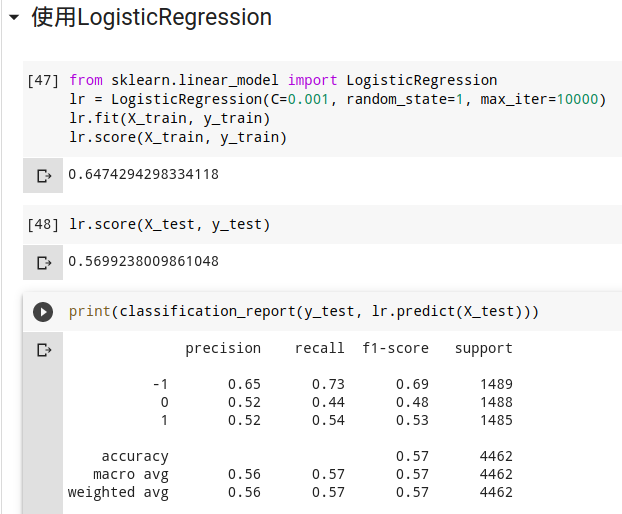
\includegraphics[width=3.5in]{asset/Logistic_word2vec.png}
    \caption{\lstinline{Logistic}回归运行结果-word2vec} 
\end{figure}

使用\lstinline{GloVe}作为词向量生成,降维后运行结果如下所示

\begin{figure}[htb]
    \centering
    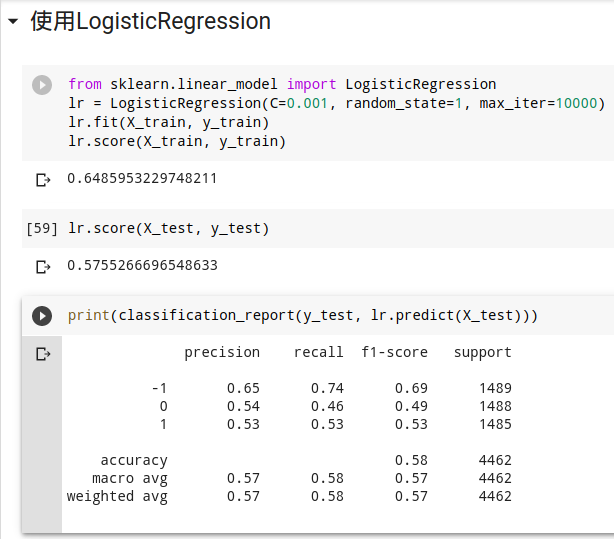
\includegraphics[width=3.5in]{asset/Logistic_glove.png}
    \caption{\lstinline{Logistic}回归运行结果-GloVe} 
\end{figure}

可见在相同配置下,\lstinline{GloVe}生成的词向量比\lstinline{CBOW}生成的词向量更加优秀,这也与业界实际情况相符。

\newpage
\subsubsection{\lstinline{SVM}}

使用\lstinline{word2vec}作为词向量生成,降维后运行结果如下所示
\begin{figure}[htb]
    \centering
    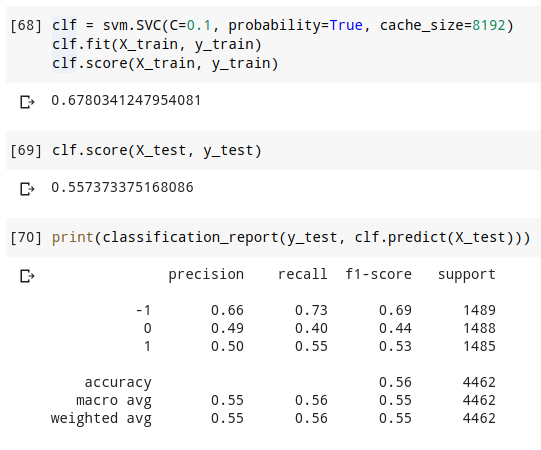
\includegraphics[width=3.5in]{asset/SVM_word2vec.png}
    \caption{\lstinline{Logistic}回归运行结果-word2vec} 
\end{figure}

使用\lstinline{GloVe}作为词向量生成,降维后运行结果如下所示

\begin{figure}[htb]
    \centering
    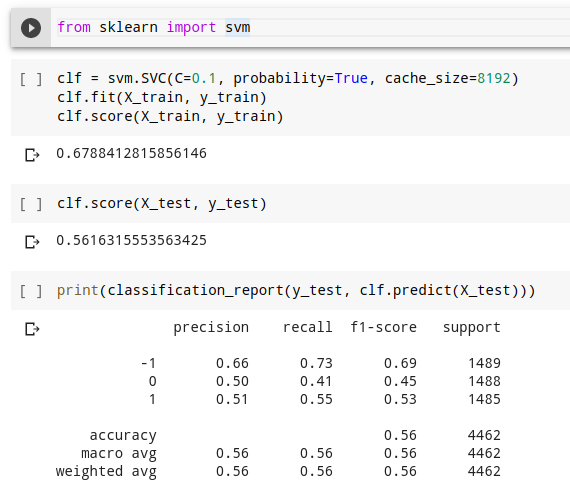
\includegraphics[width=3.5in]{asset/SVM_glove.png}
    \caption{\lstinline{Logistic}回归运行结果-GloVe} 
\end{figure}

可见不管是\lstinline{SVM}还是\lstinline{Logisitc},使用\lstinline{GloVe}生成的词向量都要更加好。
\newpage
\subsubsection{\lstinline{LSTM}}

使用\lstinline{tensorflow}构建简单的\lstinline{LSTM}模型,将转换的整数编码数据输入,设置\lstinline{epoch}为20,进行训练,如下图所示

\begin{figure}[htb]
    \centering
    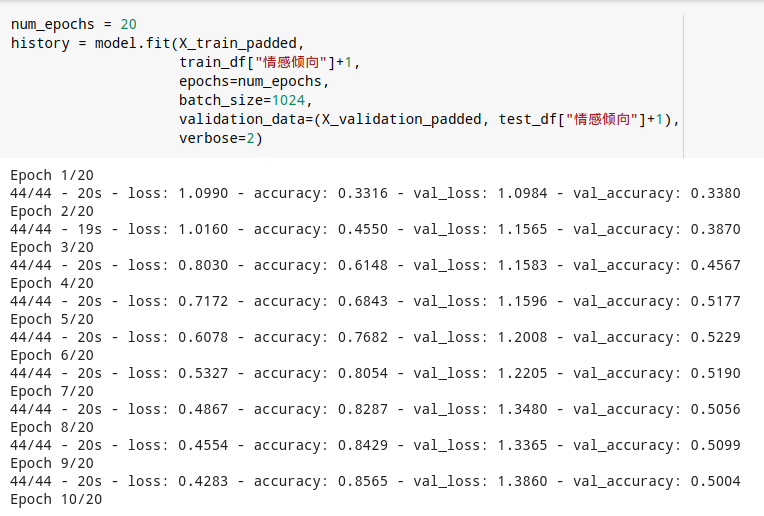
\includegraphics[width=5in]{asset/LSTM训练过程.png}
    \caption{\lstinline{LSTM}训练过程.png} 
\end{figure}

同时可以通过训练历史绘制出正确率与loss的变化曲线,如下图所示

\begin{figure}[htb]
    \centering
    \subfigure[模型正确率]{
        \begin{minipage}[t]{0.4\linewidth}
            
            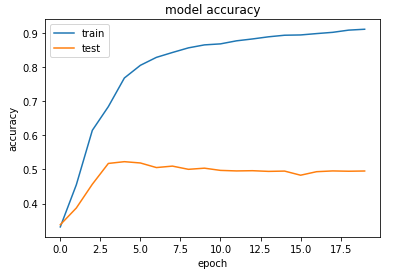
\includegraphics[width=2.5in]{asset/LSTM图1.png}
            %\caption{fig1}
        \end{minipage}%
    }%
    \subfigure[loss变化]{
        \begin{minipage}[t]{0.4\linewidth}
            
            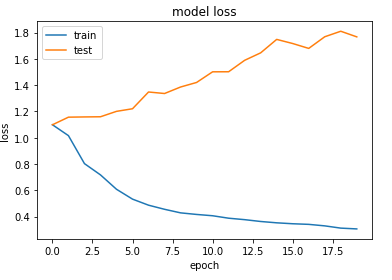
\includegraphics[width=2.5in]{asset/LSTM图2.png}
            %\caption{fig2}
        \end{minipage}%
    }%
    \caption{\lstinline{LSTM}训练变化过程}
\end{figure}

可以发现在训练过程中,在第5个\lstinline{epoch}时达到最佳状态,测试集正确率0.52,训练集正确率0.78,之后则发生了过拟合,训练集上的正确率不断增加
但测试集的正确率却进入瓶颈并有减小的趋势,其loss也不断增加。
\newpage
\subsubsection{不同方法比较}

分别列出不同模型或方法的正确率,如下表所示

\vspace*{2em}
\begin{table}[htb]
    \centering
    \begin{tabular}{cccc}
    \toprule  %添加表格头部粗线
    % 模型& \lstinline{precision}均值& \lstinline{recall}均值 \lstinline{f1-score}均值\\
    % \midrule  %添加表格中横线
    % \lstinline{Logitstic+GloVe}& 0.57& 0.58 & 0.57\\
    % \lstinline{Logitstic+word2vec}& 0.56& 0.57 & 0.57\\
    % \lstinline{SVM+GloVe} & 0.56 & 0.56 & 0.56\\
    % \lstinline{SVM+word2vec} & 0.55 & 0.56 & 0.55\\
    % \bottomrule %添加表格底部粗线
    模型& precision均值& recall均值& f1-score均值\\
    \midrule
    Logitstic+GloVe& 0.57& 0.58 & 0.57\\
    Logitstic+word2vec& 0.56& 0.57 & 0.57\\
    SVM+GloVe& 0.56& 0.57 & 0.57\\
    SVM+word2vec& 0.55 & 0.56 & 0.55\\
    LSTM& 0.50 & 0.52 & 0.50\\
    \bottomrule
    
    \end{tabular}
    \caption{不同方法的指标对比}

\end{table}

可见不同方法之间的差异不大,其中\lstinline{Logitstic+GloVe}的方法效果最好,而神经网络的方法最差。由于前者使用了词嵌入的方法,而后者只是简单的
整数编码,相较之下,后者损失了不少信息。

同时本人在实验过程中尝试将项目给出的训练集以及测试集进行重新乱序分割,其正确率可以达到0.7以上,所以有点怀疑
这个实验的测试集是不是有问题。而题目中又明确指出需要使用提供的测试集,所以最终的效果不是非常好,基本都在0.56左右。并且本项目与常规的情绪二分类有所不同
,采用的是三分类,所以就更加困难。
\newpage

\subsection{思考与总结}

\subsubsection{个人体会}
经过本次项目,我对于文本处理有了更加深刻的理解。通过查阅各种资料,甚至是看cs224n(著名自然语言处理课程)。了解了各种文本处理的方法,如数据预处理,
各种不同的数据编码方式,以及各种词向量的算法,如\lstinline{Skip-Gram}、\lstinline{GloVe}等等。也尝试了各种其他的方法,如\lstinline{tfi-df}
以及\lstinline{bag-of-word},其中有些方法效果不是非常理想所以就没有在报告中体现(可以在代码中找到)。虽然各种方法综合起来,最高的正确率只有0.57,
但是在整个学习的过程中,结合课程中学到的知识,以及实际工程上实现的过程,我对于各种模型的建立,以及各种可调节参数的调节方法都有了更深入的了解。

同时,对于在训练集上可以达到90\%以上的正确率,而在测试集上却始终无法突破60\%的情况,我也进行一些测试。发现通过混合测试集以及训练集,并重新随机分割,
正确率可以达到70\%以上。所以怀疑这个测试数据是不是有些问题。
\subsubsection{建议与意见}
个人感觉课程中学习到的知识,其实无法处理像项目一这种比较综合的项目,许多课程中学习到的模型都无法很好的在项目一中运用。当然也有其他的项目的难度与课程内容
匹配,比如项目六。也许在提供此类比较"超纲"的项目的时候,可以提供一些相关的参考资料,可以很大程度上减少我们自己毫无方向的学习。其他的方面还是比较不错的
提供了充足的时间让我们来做这些项目,老师在群里答疑也很及时。
\end{document}